\section{Introduction}
Segmentation and clustering of large amounts of data is one of the main research fields of modern artificial intelligence.

In recent years, with the expansion and diffusion of the digitalization of physical archives both in the private and public sector these branches of artificial intelligence have become increasingly prominent for economic and financial reasons since they can easily shrink the amount of man-hours needed to achieve the tasks involved. 

Related to these circumstances, the application developed in our work presents a way to group together handwritten words with the same internal structure.
Our intent is to make possible through the use of our application to group images, representing the same word, contained in handwritten scanned documents in sets with a non-banal precision.
From these sets a human operator can thus categorize all the contained words through the apposition of a single label per set, rather than per element, with obvious gains in time and costs.

  
The basis of our work is the collection of U.S. Census data of the year 1930.
Our goal is to divide enrollees by state: we do so through the clustering of the handwritten words contained in the "State" field of the form.

Document segmentation and extraction of the words corresponding to the states was developed previously by two of our colleagues in the course of \emph{Technology of Databases} for documents with a similar form to the ones of our dataset, their project is thus the starting point of our work: our main contribution to the preexisting work is in the definition of a different, more relevant, valuation method through which determine the distance between different images, in hope that.
The method proposed in our paper is the utilization of \textit{structural features}, directly connected to the stroke with which the words were written. 
The main problem on which we have worked is thus the extraction of features from handwritten words with the goal of creating clusters of similar elements in order to facilitate the recognition by a human agent.

\begin{figure}[!ht]
\centering
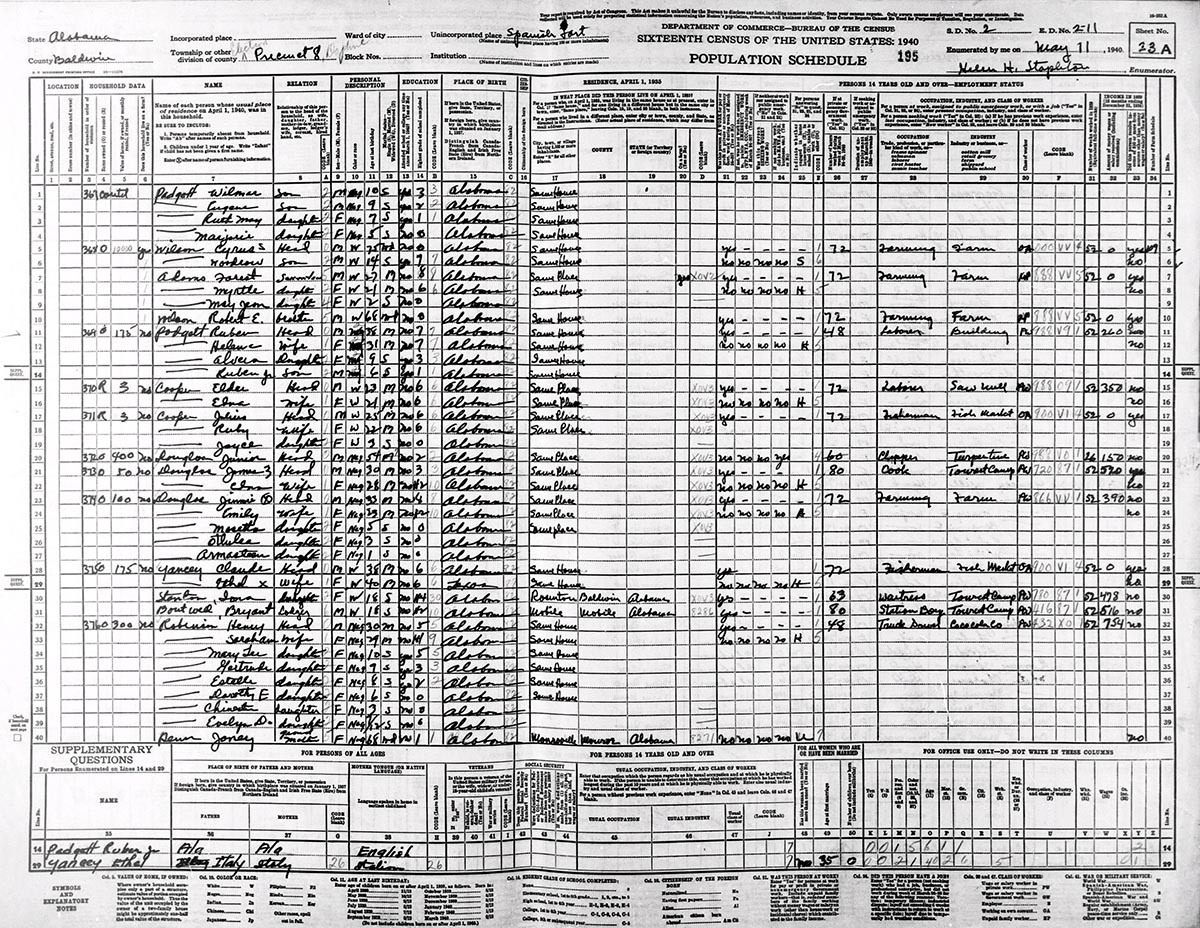
\includegraphics[width=0.66\textwidth]{images/img1.jpg}
\caption{An example of a table containing census data}
\end{figure}